\documentclass[11pt]{article}
\usepackage[tmargin=1in,lmargin=1in,rmargin=1in,bmargin=1.2in]{geometry}
\usepackage{float}

\setlength{\parindent}{0pt}
\setlength{\parskip}{0.25em}
\usepackage{setspace}
\setstretch{1.1}

\usepackage{graphicx} % Required for inserting images

\title{CS520 Project 3: Machine Learning - What Is It Good For?}
\author{Aditya Girish, Rishik Sarkar}
\date{November 10 2023}

\begin{document}

\maketitle

\section{Model 1}

This section is dedicated to our training and testing of Model 1, which is used to predict the best next move for the bot based on the current grid configuration. The subsections shall include the following essential information: the general pipeline of Model 1, a thorough analysis of the training process, and a presentation of the testing process along with any relevant results.

\subsection{Model 1 Pipeline}

I have outlined the general pipeline of Model 1 below, along with any crucial steps taken:

\begin{enumerate}
    \item Import relevant packages and run the \emph{Bot1.ipynb} notebook to gain access to all the setup functions used for Bot 1 in Project 2. None of the functions have been modified, and they allow us to set up the 30x30 grid, randomly place one bot, alien, and crew member, initialize alien and crew probability matrices, move the bot and aliens, update probability matrices, and deterministically determine the best move for the bot. Note that we fixed the ship's layout in terms of the default blocked and open cells, and only the locations of the bot, alien, and crew member change in any given simulation
    \item Simulate Bot 1 similarly to how it was done in Project 2, but collect relevant feature and output vectors to save in a Pandas dataframe (and eventually store as \emph{model\_data\_raw.csv} to be used in training Model 1. I shall go into more detail about the exact feature and output vectors in the next section.
    \begin{enumerate}
        \item To collect enough data, we ran 6000 bots (i.e., until the bot saved the crew or got captured): 30 iterations per simulation and 200 simulations
        \item Through these simulations, we collected a total of 4,132,796 data points
        \item The following hyperparameters were used: alpha = 0.004, k = 3
        \item These were the metric results from the simulation:
        \begin{itemize}
            \item Average Rescue Moves: 585.05
            \item Probability of Crew Rescue: 0.71
            \item Average Crew Saved: 21.3
        \end{itemize}
        \item Note that these values only reflect the final simulation for our data collection phase. Since we modified the input and output vectors several times after the training/testing phase, our simulation hyperparameters, data size, and metrics constantly changed
    \end{enumerate}
    \item Preprocess the collected data and perform train/test splits for the input matrix X and output vector y. We also generated a validity mask for the output vector at this pipeline step, but more later. The following general preprocessing steps were taken:
    \begin{enumerate}
        \item Read the data from \emph{model\_data\_raw.csv} and ensure that the shape is consistent and the data is loading correctly
        \item Remove duplicates from the data to streamline the dataset and remove redundancy. Without this step, the model might memorize frequently occurring data points or become skewed/biased. After this step, the total data points are reduced to 1,787,373
        \item At this point, perform any necessary adjustments to the feature vectors (i.e., dropping/adding columns, normalizing data, etc.). Since we were confident about our features during our final collection process, we did not make any modifications to the collected data
        \item Separate the data into the input matrix X and the output vector y (with the output being the last column and the input being all the other columns). Note that PCA or other feature engineering methods could also be performed in this step
        \item Divide the X and y dataframes into train and test sets with an 80/20 split, respectively. At this point, we also checked that all five classes were equally represented in each set
        \item Finally, generate the validity mask vector dataframes for the train and test sets. Each row in the validity mask corresponds to the same row in the X\_train and X\_test datasets, and essentially represents the neighbors that the bot can move to given the board's open and closed cells. The following process was used to generate this validity mask:
        \begin{enumerate}
            \item For any given datapoint, use the bot\_x and bot\_y features (that represent the bot's current coordinates) along with an empty grid state to determine what neighbor cells count as valid moves for the bot
            \item Each datapoint in the valid dataframes is represented as a list in the form of [$c_1, c_2, c_3, c_4, c_5$] depicting the up, down, left, right, and bot cells, respectively. Each $c_i$ is 0 if the corresponding relative neighbor is an invalid move and 1 if the bot can move to it. The significance of this vector will become clear in the next section
        \end{enumerate}
    \end{enumerate}
    \item Train the logistic regression model on the X\_train + y\_train dataset and save the updated W and b values for Model 1. Since I will go into the input, output, model spaces as well as the learning techniques in the next section, this point is dedicated to discussing the final training hyperparameters:
    \begin{itemize}
        \item alpha (learning rate) = 0.01
        \begin{itemize}
            \item We additionally tried 0.001 and 0.05, but 0.01 seemed to be optimal. A value of 0.001 caused the model training to be prolonged, whereas 0.05 caused the loss to fluctuate due to overstepping
        \end{itemize}
        \item epochs = 50
        \begin{itemize}
            \item We tried several other epoch values, but 50 seemed an ideal number for the loss to decrease until it became asymptotic
        \end{itemize}
    \end{itemize}
    \item Test Model 1 on the testing dataset with the updated W and b values and calculate the accuracy of predicting the best move. I shall discuss our findings in more detail in the Results section, but we generally saw no indication of overfitting and achieved decent training and testing accuracy
    \begin{itemize}
        \item Additionally, to confirm that the decrease in loss caused an increase in accuracy (i.e., the model was improving), we calculated the training and testing accuracy using randomized weights and biases and averaged the results over 100 calculations. Overall, we were able to find a significant improvement in both training and testing accuracy using the trained weights than the randomized weights, thus indicating that the model truly learned
    \end{itemize}
    \item Simulate Model 1 through a new bot called Mimic-Bot1 that utilizes the logistic regression model's predictions to determine the next move for the bot by utilizing the same features as the trained model. Here is a general outline of the process:
    \begin{enumerate}
        \item Create the Mimic-Bot1 simulation function identical to the Bot1 simulation function, but instead of using the deterministic \emph{determine\_move()} function defined in \emph{Bot1.ipynb}, predict the next move at each timestep by using Model 1 with a dataframe input containing features extracted from the current ship configuration (similar to the data collection function)
        \item Test the Mimic-Bot1 simulation out against the Bot1 simulation function similar to how the testing was performed in Project 2 with Bot 1 and Bot 2, and store the collected average metrics for each bot
        \item We ran 400 bots for both Bot 1 and Mimic-Bot1: 20 iterations per simulation and 20 simulations
        \item The following hyperparameters were used: alpha = 0.004, k = 3
        \item Importantly, we calculated a validity mask for every X input, and used a prediction function that applied the validity mask to the output to ensure that the bot would remain within bounds
        \item Later, we added a stochastic element to the prediction provided by Model 1. In essence, we generated a random number between 1 and 5 and returned a random valid move if the number was 1 (i.e., 20\% of the time). This modification accounted for situations where Mimic-Bot1 got stuck in an endless loop. Consider the following scenario: The bot is in a cell from which the highest probability neighbor is "up," but following the highest probability from "up," the bot is taken back to the original cell. By adding slight randomness, Mimic-Bot1 can escape such loops by taking unexpected actions
    \end{enumerate}
\end{enumerate}

\subsection{Training Process}

In this section, I shall outline the training process for Model 1, including the input and output features, the model space, the loss function, and the training algorithm we used.

\subsubsection{Input Space}

The data that was collected and represented as input features in our final model are as follows:

\begin{enumerate}
    \item The bot's current x and y coordinates as two individual integer features \emph{bot\_x} and \emph{bot\_y}
    \begin{itemize}
        \item Previously, we naively tried storing this feature as a string of a tuple but realized that separating the coordinates into two numerical features was the only way we could use logistic regression since they must be multiplied by weights
        \item We also once tried removing the features altogether, but we achieved better accuracy by including them
    \end{itemize}
    \item The alien probabilities for all neighboring cells (and the current bot cell) as float32 features. They are in the order: \emph{alien\_up}, \emph{alien\_down}, \emph{alien\_left}, \emph{alien\_right}, \emph{alien\_stay} representing the probabilities of the alien being in the up, down, left, right, and bot cells respectively. We tried several other versions for the alien probabilities, as outlined below:
    \begin{itemize}
        \item At first, we included the entire flattened alien probability matrix (which was stored as a dictionary in the simulation), which meant that every individual open cell key within the dictionary was represented by a feature in the form \emph{alien\_[str(key)]} with the probability value stored as a float64 (and later float32). This approach resulted in around 1,219 features (including the others), which caused our data collection phase to take an extremely long time and resulted in an 18 GB CSV dataset!
        \item Understanding that the professor mentioned a similar approach within office hours and that having as much information as possible could not hurt, we attempted the entire training, testing, and simulation process with this expansive dataset, only to find that the accuracy was still very low. I dove into the simulation results and the calculated weights to resolve this issue (and potentially streamline the process). I realized that a significant problem was the low variance between the values of each feature over all datapoints and a predominance of tiny and zero probabilities. To resolve this, I attempted to filter out and keep only features with variance above a certain threshold (0.01, 0.001, 0.0001, etc.) but did not see a significant change over several training and testing periods.
        \item As a last resort, I even attempted to use Principal Component Analysis (PCA) for dimensionality reduction by following these steps:
        \begin{enumerate}
            \item Standardized data and computed the covariance matrix
            \item Performed eigenvalue and eigenvector decomposition and sorted eigenvalues in descending order
            \item Selected the top 10, 100, and 200 eigenvectors (over three different tests)
            \item Transformed the original dataset based on the projection onto the relevant eigenvectors
        \end{enumerate}
        However, I ran into issues with the eigenvector computations due to the low variance in the dataset (all PCs contained 0s for any sub-dataset with over 50,000 datapoints and \emph{k\_components} = 100), and I was not sure how to reflect the projection onto the collected datapoints during the simulation, so we chose to abort the process ultimately
        \item Finally, looking into the process we utilized in deterministically finding the best next move in Project 2, we decided only to consider the up, down, left, right, and current cells, which also significantly improved the data collection efficiency, reduced the CSV file size and allowed for more datapoints, and increased the overall training and testing accuracy. To account for the low probabilities within the remaining five alien probability features, we normalized them so that they summed up to 1 (unless their sum was 0 before)
    \end{itemize}
    \item The crew member probabilities for all neighboring cells (and the current bot cell) as float32 features. They are in the order: \emph{crew\_up}, \emph{crew\_down}, \emph{crew\_left}, \emph{crew\_right} representing the probabilities of the crew member being in the up, down, left, and right cells respectively. All the variations that we tried out for alien probabilities were also applied to the crew probabilities, with a few changes:
    \begin{itemize}
        \item We decided to drop the \emph{crew\_stay} column since the crew probability was guaranteed to be 0 for the bot's current cell. We attempted to remove the corresponding \emph{alien\_stay} column as well, but saw no significant improvement in performance or accuracy
        \item Note that crew member probabilities were typically higher than alien probabilities since the only situations where alien probabilities were high were when the alien was within the detection square sensor, whereas crew probabilities were likely non-zero. Thus, normalizing crew probabilities seemed to have a more significant impact than alien probabilities
    \end{itemize}
    \item Per the professor's announcement, we added features reflecting the distance from the bot's neighboring cells to the two cells with the highest alien and crew member probabilities, respectively. Hence, we included ten additional features: \emph{d\_alien\_up}, \emph{d\_alien\_down}, \emph{d\_alien\_left}, \emph{d\_alien\_right}, \emph{d\_alien\_stay}, \emph{d\_crew\_up}, \emph{d\_crew\_down}, \emph{d\_crew\_left}, \emph{d\_crew\_right}, \emph{d\_crew\_stay} stored as float32 values. To collect these features, we had to modify our simulation function slightly and add two new helper functions:
    \begin{itemize}
        \item We initially found the key cell with the highest probability for the crew and alien matrices and then calculated the distance from each direction cell to the respective max probability cells (if the direction cell was open). Instead of running BFS every time, we utilized the crew sensor function defined in Project 2 (without actually storing the crew detection results) and saved the \emph{d\_list} for the open direction cell within the \emph{d\_lookup\_table} to make the simulation more efficient 
        \item To recap, the \emph{d\_lookup\_table} dictionary stores cell tuples as keys and the distances to all other open cells as their respective values in the form of dictionaries. We did this so that the distance dictionary (i.e., \emph{d\_dict}) did not need to be recalculated using BFS every time. Using the crew sensor and updating the \emph{d\_lookup\_table} improved the efficiency of the distance determination process and the entire simulation
        \item After collecting the distance values for all direction cells from the max alien and crew probability locations, we stored the feature values as $1/$\emph{d\_direction\_cell} if the direction cell was open, and 0 if not
        \item Since we did not use the actual alien and crew member locations within our calculation process or as features, I am confident that we met the criteria of the project
    \end{itemize}
    \item The binary values for whether the bot received a beep or not from the alien sensor and crew sensor as two features: \emph{alien\_detected} and \emph{crew\_detected}
    \begin{itemize}
        \item The values for the features are 0 if the corresponding sensors return False and 1 if they return True
        \item Although these did not make much sense to include at first, removing them caused the accuracy to decrease. This illogical result might have occurred because of the sparsity of the dataset and the model learning from features with more variance, such as these two. We kept the features, however, and have not observed a decrease in accuracy, especially after adding in the new features introduced above
    \end{itemize}
\end{enumerate}

Overall, our final Model 1 was trained on 23 distinct features stored as integers and float32 values, as depicted above.

\subsubsection{Output Space}

The output space for Model 1 consisted of the best move made by the bot with a given ship configuration. The only thing that changed was how it was encoded:

\begin{itemize}
    \item At first we naively tried to store the output value as a string encoding of the tuple cell. In hindsight, this was clearly not the correct technique, since it would have to be predicted from a combination of numerical weights and input vectors
    \item Then, we tried to encode the output values as integers from 1 to 5, with 1 = up, 2 = down, 3 = left, 4 = right, and 5 = stay in place. This process seemed fine at first, but it had two issues. Firstly, the model might find implicit relationships between two such output values. For example, 1 + 2 = 3, but up + down is not left. I don't even know what that means. Similarly, the model might define a sense of ordinality between the output classes, such as 1 $<$ 2 $<$ 3. These relationships could be dangerous to the training process
    \item Ultimately, we decided to one-hot-encode the output value as a list with five binary values. In this case, up = [1,0,0,0,0], down = [0,1,0,0,0], left = [0,0,1,0,0], right = [0,0,0,1,0], stay = [0,0,0,0,1]. This conversion allowed us to introduce a linear relationship between all the classes and removed the possibility of unnecessary dependencies. Also, one-hot-encoding allowed us to make the validity mask generation and application process much simpler during the loss and gradient calculation and prediction phases
    \item Within the CSV itself, the one-hot-encoded output values are stored within double quotes, but the dataset loading process ensures that the output vector is one-dimensional and contains the list of encodings per datapoint
\end{itemize}

\subsubsection{Model Space}

To map from the input to the output, we considered a multiclass logistic regression model with softmax activation. Essentially, here are the steps followed by the logistic regression model:

\begin{enumerate}
    \item During training, the model receives an input vector $X_i$, and uses a linear combination of the vector with weights (W) and bias (b) to compute the output $z = X_i \cdot W + b$
    \item The output is then transformed into probabilities for each class via the softmax function. Essentially, the probability for class with index $i$ given the output value, and the fact that there are 5 classes (up, down, left, right, stay), is computed as such:
    \begin{itemize}
        \item softmax($z_j) = \frac{e^{z_j}}{\sum_{i=1}^{5} e^{z_i}}$
    \end{itemize}
    This ensures that the probability is distributed over the 5 possible moves
    \item Bonus:
    \begin{itemize}
        \item For our bonus, we used the scikit-learn \emph{LogisticRegression} library to create a multiclass model using a \emph{saga} (Stochastic Average Gradient Augmented) solver due to the extensive training dataset. The scikit-learn model also uses the softmax activation function I mentioned earlier and uses L2 regularization to prevent overfitting (which we shall go into more detail about in the next section). We used the same dataset as the logistic regression model we built from scratch. We used 1000 iterations in our training, and all the other processes were identical unless noted otherwise
    \end{itemize}
\end{enumerate}

\subsubsection{Loss}

As a multiclass classification model, Model 1 uses a cross-entropy loss function that measures the difference between the true and predicted probability distributions for the classes in the following way:

\begin{enumerate}
    \item As parameters, we input the predicted \emph{chosen\_action} vector and the true \emph{chosen\_action} vector as well as the validity mask that, as mentioned in Section 1.1, is one-hot-encoded to depict the valid moves for the bot
    \item At first, the validity mask vector is element-wise multiplied by the predicted probability vector $\hat{y}$. This operation is done so that the probabilities for invalid bot moves become 0. Then, the probabilities in $\hat{y}$ are normalized, so the sum remains 1. This process is crucial since it aligns the learning process of Model 1 with the constraints imposed by the simulation
    \item After that, the cross-entropy loss is calculated for each one-hot-encoded datapoint (with five classes) in true output vector $y$ and predicted output vector $\hat{y}$ by using the following equation:
    \begin{itemize}
        \item $L(y, \hat{y}) = - \Sigma_{i=1}^{5} y_i \cdot log(\hat{y_i} + \epsilon)$
        \item In this case, $\epsilon$ refers to a small constant (1e-15) to ensure that log(0) is not being calculated, and $L(y,\hat{y})$ is the loss for that particular datapoint
    \end{itemize}
    \item Finally, the loss for each datapoint is added up and averaged (divided by n, where n is the number of datapoints). Since the calculations take place for the entire vectors at once, this operation is implicit
    \item Bonus:
    \begin{itemize}
        \item We did not define the loss function explicitly since we used the default scikit-learn \emph{LogisticRegression} library. However, as mentioned earlier, we used L2 regularization, which, as I understand it, added a penalty to the loss function equal to the sum of the squared values of the calculated weights with a specific regularization strength. Additionally, we used L2 over L1 regularization because we found through research that L1 is better for feature selection, but since we already have very few features (after reducing the original 1,219 features to 23), L2 seemed to be a better fit for the use case
        \item Note that because we could not figure out how to account for one-hot-encoded output vectors within scikit-learn, we were forced to use integer representations for each output class (based on the index in the one-hot-encoding). For example, up = 0, down = 1, and so on. We were also unable to apply the validity mask during loss calculations, instead opting to use it only during the simulation
    \end{itemize}
\end{enumerate}

\subsubsection{Training Algorithm}

The training algorithm for Model 1 uses gradient descent to minimize the cross-entropy loss function. The algorithm iteratively updates the weights and biases to yield the lowest possible loss value. Here are the steps we followed to implement it:

\begin{enumerate}
    \item As parameters, we input the predicted output vector $\hat{y}$, the true output vector $y$, the input matrix $X$, as well as the validity mask mentioned earlier
    \item Similar to the loss function, we first multiply the validity mask vector by the predicted probability vector $\hat{y}$ to reduce invalid moves to 0 and then subsequently normalize the valid probabilities so that the sum is 1
    \item Then we calculate the gradient of the loss function with respect to the weights $W$ and bias $b$ as follows:
    \begin{itemize}
        \item $\nabla_{W} L = \frac{1}{n} X^{T} \cdot (\hat{y} - y)$
        \item $\nabla_{b} L = \frac{1}{n} \Sigma_{i=1}^{n} (\hat{y_i} - y_i)$
    \end{itemize}
    In this case, $X$ is the input matrix of size $n \times m$, and $\hat{y}$ and $y$ are the predicted and true output vectors of size $n \times 5$ (since there are five classes in the one-hot-encoding). Additionally, $L$ is the loss function that was calculated earlier
    \item Finally, after we have calculated the gradient of the loss function with respect to both $W$ and $b$, we can use them to update the weights and bias in the following way:
    \begin{itemize}
        \item $W = W - \alpha \cdot \nabla_{W} L$
        \item $b = b - \alpha \cdot \nabla_{b} L$
    \end{itemize}
    The $\alpha$ used in these updates refers to the learning rate of the training algorithm (which we set to 0.01) for our final training. We tested out with several $\alpha$ values and found that smaller values led to much slower convergence, whereas larger values made the loss oscillate instead of steadily decreasing sometimes (indicating that the updates were overstepping and missing the minimum)
    \item We utilized this algorithm in each iteration or epoch to train the model on the entire dataset. We previously tried out stochastic gradient descent by updating the parameters for smaller batch sizes to improve convergence speed (later switching to regular gradient descent after a specified loss difference threshold). However, we realized that the loss function decreased more steadily by utilizing full-batch gradient descent the entire time. Overall, we finally trained Model 1 for a total of around 50 epochs, which allowed the loss to decrease and eventually become asymptotic
    \item Bonus:
    \begin{itemize}
        \item Once again, we did not explicitly define the training function since we used the default scikit-learn \emph{LogisticRegression} library. As mentioned earlier, we utilized \emph{saga}, or Stochastic Average Gradient Descent, which uses the same process defined earlier, albeit much more efficiently, for faster convergence. Additionally, we set the total number of epochs to 1000 to ensure loss convergence
    \end{itemize}
\end{enumerate}

\subsection{Testing Process and Results}

This section will highlight our training, testing, and simulation results and an overall analysis of our findings.

\subsubsection{Results}

Here are a few of the loss function plots we generated during training:

\begin{itemize}
    \item Figure 1 shows the decrease in the loss function using Stochastic Gradient Descent. Notice that the initial loss was very high, and despite decreasing steadily, showed minor improvement in accuracy

% \begin{figure}[H]
%     \centering
    % 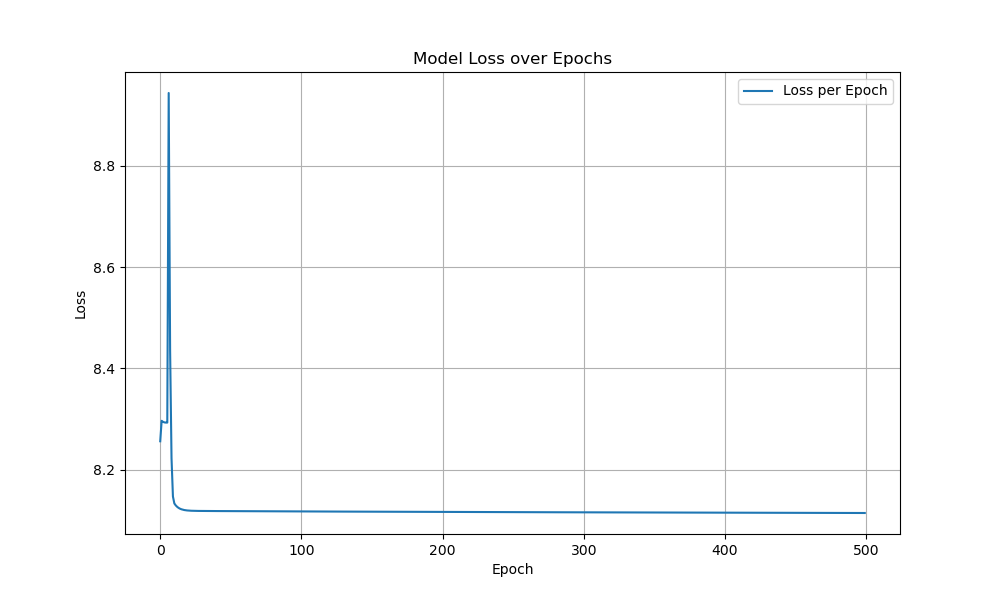
\includegraphics[width=0.8\linewidth]{loss_sgd.png}
%     \caption{Loss Function using SGD}
% \end{figure}
    
    \item Figure 2 shows the problem of using a higher $\alpha$ value of 0.1. The loss function continuously fluctuated due to overstepping the minimum, and the model did not learn

% \begin{figure}[H]
%     \centering
%     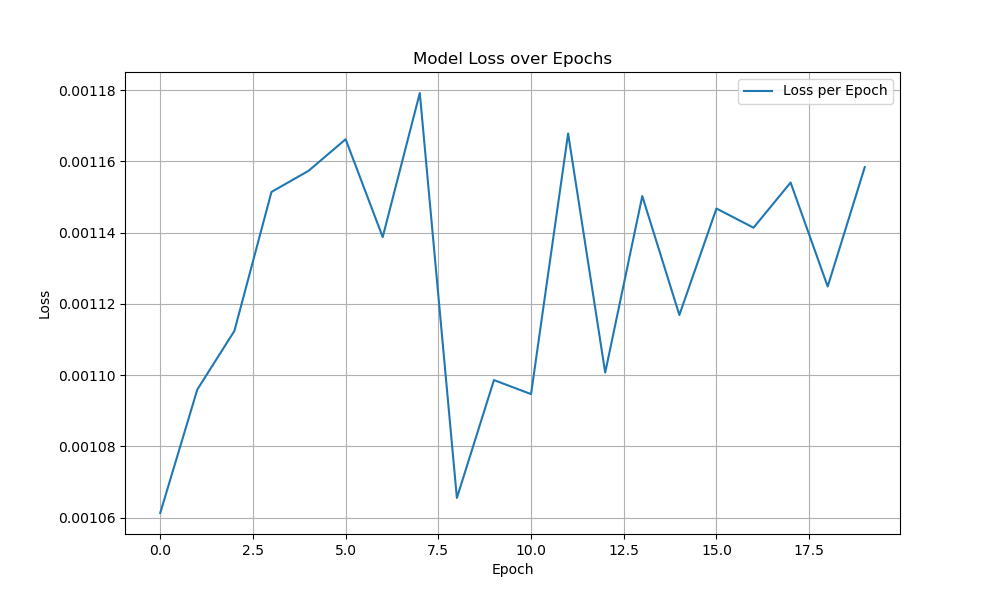
\includegraphics[width=0.8\linewidth]{loss_highalpha.png}
%     \caption{Loss Function with alpha=0.1}
% \end{figure}
    
    \item Figure 3 shows the final loss function we achieved through training Model 1. The loss decreases and gradually becomes asymptotic, indicating that the model was learning over time. Despite the apparent improvement in accuracy and decreased loss, we noticed the loss value was exceptionally low (even though further testing showed no indication of the model memorizing features). We found this very confusing and eventually realized that this was because our feature values were mostly sparse with many 0s, so the model was learning as much as it could, given the data. We tried training the model on the dataset with 1,219 features and the ones after PCA and variance threshold filtering but did not see a difference in the calculated loss. Overall, as we shall depict in the following section, we tested the model's accuracy using trained and random weights and biases and saw that the model learned adequately, so the abnormally low loss value did not affect Model 1 negatively
\end{itemize}

% \begin{figure}[H]
%     \centering
%     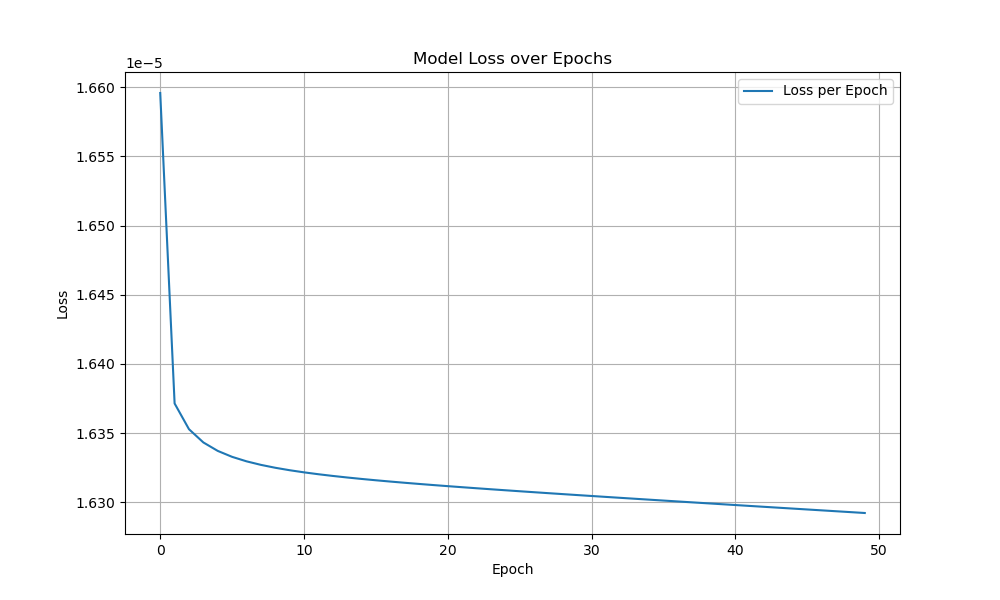
\includegraphics[width=0.8\linewidth]{loss1.png}
%     \caption{Final Loss Function}
% \end{figure}

\subsubsection{Testing and Evaluation}

After training the model on 50 epochs and ensuring that the loss function had decreased sufficiently, we tested Model 1 on the training and test datasets containing 1,429,898 and 357,475 datapoints respectively. Here are our findings using the \emph{predict\_constrained()} function that applies the validity mask to the predicted probabilities and returns the move class with the maximum probability:

\begin{itemize}
    \item Training Accuracy: 0.7017115906169531
    \item Testing Accuracy: 0.7074145045108049
\end{itemize}

Now, this might not initially seem like a lot and begs the question: what if the model randomly predicts outputs instead of having learned the optimal weights? To counter this argument, we devised an algorithm to generate 100 random weight and bias vectors and calculate the testing accuracy using each parameter pair. We then found the maximum and minimum testing accuracies from the test and compared them to the testing accuracy of the learned parameters:

\begin{itemize}
    \item Maximum Random Testing Accuracy: 0.4941895237429191
    \item Minimum Random Testing Accuracy: 0.4485997622211344
\end{itemize}

Since 0.707 $>$ 0.494, the maximum random testing accuracy over 100 trials, we can affirm with reasonable certainty that Model 1 has indeed learned optimal weights and biases over the training period.

Now, what about whether the model is overfitting or not? Firstly, we have shown that the training and testing accuracy are virtually identical (with the testing accuracy being slightly higher). This finding indicates that the model has not overfitted the training dataset since it performs just as well on the testing dataset. Since the datasets themselves are quite large, we should be able to confirm that the model does not overfit significantly.

However, what if the model has just memorized the bot location features and often predicts the same output since the board configuration was relatively homogenous over the same simulation trial we used to collect data? To answer this question, we tried generating five other test datasets with randomized board start states (in terms of bot, alien, and crew locations) and got similar accuracy values to the training accuracy we found with the original dataset. For example, one of our testing datasets returned an accuracy of 0.7146513365126948, even higher than the testing accuracy on the original dataset. None of our testing datasets returned a lower accuracy than the training accuracy, indicating that the model was not overfitting much and is reasonably generalizable.

\subsubsection{Bot1 vs. Mimic-Bot1}

In this section, we will talk about some specific setups of the Mimic-Bot1 simulation function (along with helper functions) and evaluate the overall performance of Model 1 in practice:

\begin{itemize}
    \item Our Mimic-Bot1 function was almost identical to the Bot1 function defined in Project 2 (and the data collection function defined earlier), but the main difference was the algorithm to predict the next move for the bot given a ship state. Within Bot1, the prediction occurs deterministically, using the logic-based function defined in Project 2 that returns the highest probability neighbor with a 0 alien probability. However, for Mimic-Bot1, the prediction function takes in as parameters the features used in training Model 1 and outputs the model's prediction in the form of a tuple reflecting the best next move
    \item The best-move-finding function initially utilized the \emph{predict\_constrained()} function defined earlier that applies the validity mask to Model 1's predictions based on the input X and returns the highest probability valid neighbor. However, as mentioned earlier, we modified this approach slightly to incorporate a stochastic element in move prediction to avoid endless loops by the bot in some specific scenarios
    \item In the evaluation, we used the same three metrics in Project 2: Average Rescue Moves, Probability of Crew Rescue, and Average Crew Saved. For the hyperparameters, we used the same values as the data collection function: alpha = 0.004, k = 3, timeout = 10,000, with 400 bots for both Bot1 and Mimic-Bot1
    \item Overall, Mimic-Bot1 performed similarly to Bot1 sometimes but was sometimes worse. Here are the results we collected over the span of 20 trials (each containing the average metrics for 20 bots for Bot1 and Mimic-Bot1):
    \begin{itemize}
        \item Bot1: {Average Rescue Moves: [627.05]}, {Probability of Crew Rescue: [0.73]}, {Average Crew Saved: [14.6]}
        \item Mimic-Bot1: Bot1: {Average Rescue Moves: [1768.05]}, {Probability of Crew Rescue: [0.42]}, {Average Crew Saved: [8.4]}
    \end{itemize}
    \item These results suggest that, on average, Bot1 performed significantly better than Mimic-Bot1, but Model 1's predictions weren't completely useless. The large average number of required moves for rescues directly affected the loops that the mimic bot often found itself in, which weren't wholly mitigated despite the addition of stochasticity. Mimic-Bot1 was limited in performance to Bot1's capability since Model1 was trained on simulations using Bot1 itself. Overall, Mimic-Bot1 displayed the ability to traverse the ship effectively and rescue crew members while avoiding aliens, albeit not as well as its deterministic counterpart
\end{itemize}

\section{Model 2}

% \subsection{Input}

% \subsection{Model}

% \subsection{Training}

% \subsection{Error}

% \subsection{Output}

\section{Model 3}

% \subsection{Input}

% \subsection{Model}

% \subsection{Training}

% \subsection{Error}

% \subsection{Output}

\end{document}
